\documentclass{standalone}

\usepackage{tikz}

\usetikzlibrary{positioning, chains, shapes.geometric, fit, shapes, arrows.meta, calc}

\begin{document}

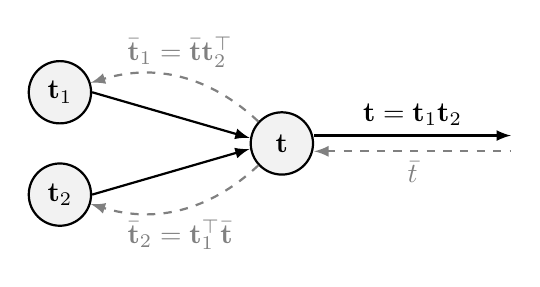
\begin{tikzpicture}[
    >=LaTeX, % Use default LaTeX arrows
    % Styles 
    node/.style={ % Input or output node
        circle,
        minimum width=2.25em,
        draw,
        fill=gray!10,
        thick
    },
    arrow/.style={
        -latex,
        thick
    },
    backprop/.style={ % Backpropagation arrows
        arrow,
        dashed,
        gray
    }
]
    % Computational graph nodes
    \node[node] (t) {$\mathbf{t}$};
    \node[node] (t1) [left=of t, xshift=-1cm, yshift=0.65cm] {$\mathbf{t}_1$};
    \node[node] (t2) [left=of t, xshift=-1cm, yshift=-0.65cm] {$\mathbf{t}_2$};

    % Computational graph edges
    \draw[arrow] (t1.east) -- ([yshift=2pt]t.west);
    \draw[arrow] (t2.east) -- ([yshift=-2pt]t.west);
    \draw[arrow] (t.east) +(0cm,0.1cm) -- +(2.5cm,0.1cm) node[midway, above] {$\mathbf{t} = \mathbf{t}_1 \mathbf{t}_2$};

    % Backpropagation arrows with partial derivatives
    \draw[backprop, bend right] (t) to node[midway, above] {$\bar{\mathbf{t}}_1 = \bar{\mathbf{t}} \mathbf{t}_2^\top$} (t1);
    \draw[backprop, bend left] (t) to node[midway, below] {$\bar{\mathbf{t}}_2 = \mathbf{t}_1^\top \bar{\mathbf{t}}$} (t2);
    \draw[backprop, latex-] (t.east) +(0cm,-0.1cm) -- +(2.5cm,-0.1cm) node[midway, below] {$\bar{t}$};
\end{tikzpicture}

\end{document}